\documentclass[11pt]{amsart}
\usepackage{geometry}                % See geometry.pdf to learn the layout options. There are lots.
\geometry{letterpaper}                   % ... or a4paper or a5paper or ... 
%\geometry{landscape}                % Activate for for rotated page geometry
%\usepackage[parfill]{parskip}    % Activate to begin paragraphs with an empty line rather than an indent
\usepackage{graphicx}
\usepackage{amsmath}
\usepackage{amssymb}
\usepackage{epstopdf}
\usepackage{epsfig}
\DeclareGraphicsRule{.tif}{png}{.png}{`convert #1 `dirname #1`/`basename #1 .tif`.png}

\title{Scientific Computing Final Project}
\author{Howard Jing, Sun Hyoung Sonya Kim}
\date{December 25, 2011}                                           % Activate to display a given date or no date

\begin{document}
\begin{abstract}
This project discusses an algorithm called Single-Pass Algorithm which has the advantage of only requiring one access to a given matrix A. This is useful when computing very large matrices where the cost of accessing the matrix is high. For instance, if a matrix is too large to be stored in RAM, it must be accessed from other sources, such as the hard drive. Since hard drive access times are hundreds of times slower than ram, it is convenient to develop a method which only needs to access the given matrix once in order to process information about the matrix. Applications of Single-Pass algorithm include PageRank, which computes the dominant eigenvalue of a sparse matrix. This sparse matrix contains discrete probabilities that assigns the level of "importance" to the webpages. We compare and contrast various methods of solving the dominant eigenvalue problem and test the efficiency and accuracy of Single-Pass algorithm. 

\end{abstract}
\maketitle

\section{Introduction}
Much of scientific computing is concerned with constructing and implementing algorithms to solve mathematical problems. From it arises the topic of speed and efficiency; as seen throughout the course, there exists a variety of methods with varying degrees of efficiency that are used to solve the same problem. For example, with iterative methods, we are concerned about operation count per iteration and how fast the algorithm converges. However, when evaluating the total efficiency of an algorithm, we must look at time complexity as well as space complexity. The consideration of storage locations of data and the conscious effort to optimize the time taken to access the data from its storage location can certainly ameliorate the quality of the algorithm. 

Consider the problem of computing the dominant eigenvalue of a large matrix. Many times, the given matrix is small enough to fit into RAM, so the cost of accessing this matrix is very low. However, when dealing with a large matrix that needs to be stored in the hard drive, the cost of accessing the matrix to proceed with necessary computations will be very high. Therefore, this motivates us to find a modified algorithm which minimizes the number of times the algorithm passes over the given matrix in order to perform eigenvalue approximation. 

In section 2, we introduce and elaborate on the traditional methods known for computing the largest eigenvalue of a given matrix. Then in section 3, we discuss a probabilistic algorithm called a Single-Pass Algorithm which takes space complexity into consideration and carries out the calculations with just a single pass over the data. In section 4, we test out the algorithms and determine the relative efficiency of each of the methods. Lastly, in section 5, we simulate a real life application of the single-pass algorithm on a sparse matrix, motivated by the Google's link analysis algorithm, PageRank. 

\section{Classical Algorithms for Dominant Eigenvalue Problem}
Many iterative algorithms for solving the dominant eigenvalue problem are known. Among the most popular are power iteration, inverse iteration, and Raleigh quotient iteration. 

\subsection{Power Iteration}

The power iteration algorithm is a method of computing the dominant eigenvalue of a matrix $A$ $\in \mathbb{C}^{n \times n}$. Assuming that $A$ has n distinct eigenvalues, it can be factorized in the form of $A = V \Lambda V^{-1}$, where $\Lambda$ is a diagonal matrix with eigenvalues $\lambda_1 ,..., \lambda_n$. Furthermore, assume that the eigenvalues are ordered from largest to smallest, $|\lambda_1| > |\lambda_2| > ... > |\lambda_n|$, meaning that $\lambda_1$ is the largest eigenvalue, while $\lambda_n$ is the smallest eigenvalue.

Note that: 
\begin{align*}
	&A = V\Lambda V^{-1} \\
	\implies &A^k = (V\Lambda V^{-1})(V\Lambda V^{-1})...(V\Lambda V^{-1}) = V\Lambda ^k V^{-1} \\	
	\implies &A^kV = V\Lambda ^k
\end{align*}
Suppose we have a vector $x = V \hat{x} $ $\in$ $\mathbb{C}^{n \times n}$, then because $\Lambda$ is a diagonal matrix, we have that:
\begin{align*}
	A^kx &= A^kV\hat{x} \\
	& = (V\Lambda ^k)\hat{x}  \\
	& = \Sigma^{n}_{i=1} v_i \lambda_i \hat{x}_i \\
\end{align*}
Pulling out the dominant eigenvalue $\lambda_1^k$, we have that:
\begin{align*}
	A^kx = \lambda_1^k(\sum_{i=1}^n v_i \frac{\lambda_i}{\lambda_1}^k \hat{x}_i)
\end{align*}
and since for $i > 1$ we know that $|\frac{\lambda_i}{\lambda_1}| < 1$, we see that $(\frac{\lambda_i}{\lambda_1})^k \rightarrow 0$ as $k$ grows large.
This implies that as $k$ grows large, 
\[ 
	A^k x \approx \lambda_1^k v_1 \hat{x}_1
\]
which implies the power iteration algorithm,
\[
	x_{k+1} = \frac{Ax_k}{||Ax_k||}
\]
since
\[
	\frac{Ax_k}{||Ax_k||} = \frac{A^kx_0}{||A^kx_0||}
\]
This can be seen by induction.
The base case is true by definition:
\[
	x_2 = \frac{Ax_0}{||Ax_0||} = \frac{A^1x_0}{||A^1x_0||}
\]
The induction hypothesis is then:
\[
	x_{k+1} = \frac{Ax_k}{||Ax_k||} = \frac{A^kx_0}{||A^kx_0||}
\]
Then by applying the algorithm, we get that:
\begin{align*}
	x_{k+2} = \frac{Ax_{k+1}}{||Ax_{k+1}||} &= \frac{A(\frac{A^kx_0}{||A^kx_0||})}{||A(\frac{A^kx_0}{||A^kx_0||})||}\\
	&= \frac{1}{||A^kx_0||}A^{k+1}x_0(||A^{k+1}x_0||\frac{1}{||A^kx_0||})^{-1} \\
	&=\frac{A^{k+1}x_0}{||A^{k+1}x_0||}
\end{align*}
So the formula is proved. As k increases, the algorithm will converge towards the eigenvector associated with the matrix $A$'s dominant eigenvalue. Note that if $\frac{\lambda_i}{\lambda_1}$ is near one, then the algorithm will converge very slowly. However, if $\lambda_1$ is much larger than the rest of the eigenvalues, then the algorithm will converge at a reasonable rate. 

\subsection{Inverse Iteration}
If an invertible $n\times n$ matrix A has eigenvalues $\lambda_1,...,\lambda_n$ , then its inverse $A^{-1}$ has eigenvalues $\frac{1}{\lambda_1}$,..,$\frac{1}{\lambda_n}$. If we run the power iteration algorithm on the matrix $A^{-1}$, we can then find the smallest eigenvalue $\lambda_n$ of the matrix A. This process can in fact be generalized to find any eigenvalue of the matrix A.

The spectral mapping theorem states that for every $n\times n$ matrix A and every polynomial $p(x)$, if A has an eigenvalue $\lambda_i$, then $p(A)$ has an eigenvalue $p(\lambda_i)$. Then the matrix $B := A - \mu I$ has eigenvalues of $\{\lambda_1 - \mu,...,\lambda_n - \mu\}$. If $\mu$ is chosen to be very close to the arbitrary eigenvalue $\lambda_i$, then the corresponding eigenvalue $\lambda_i - \mu$ will be the smallest eigenvalue of the matrix $B$.

By applying the power iteration algorithm on the matrix $B^{-1}$, we thus arrive at the inverse iteration algorithm: 
\[
	x_{k+1} = \frac{(A-\mu I)^{-1}x_k}{||(A-\mu I)^{-1}x_k||}
\]
which converges to the eigenvalue of $A$ that is closest to the given estimated eigenvalue $\mu$. Unlike the power iteration algorithm, which only computes the dominant eigenvalue of the matrix $A$, the inverse iteration algorithm is more flexible as it can be used to compute an arbitrary eigenvalue of the matrix $A$.

However the inverse iteration method is more costly than the power iteration method. This is because at each iteration step, either a system of linear equations must be solved, or the inverse matrix must be calculated. This implies that each step of the inverse iteration algorithm costs $O(n^3)$ operations. Similar to the power iteration algorithm, the matrix A must be accessed once at each iteration, for a total of of n times. 



\subsection{Rayleigh Quotient Iteration (RQI)}
The Rayleigh quotient iteration method is similar to the inverse iteration method, but differs in that it uses an improved eigenvector estimate at each iteration to find increasingly good eigenvalue estimates. At each iteration, the Rayleigh quotient is computed to  yield a better eigenvalue estimate for the next step. We calculate the next eigenvector approximation $x_{k+1}$ by :
\[
x_{k+1} = \frac{(A-\mu_{k}I)^{-1}x_k}{||(A-\mu_{k}I)^{-1}x_{k}||}
\]
where A is the given matrix, I is the identity matrix and Rayleigh quotient $\mu_k$ is defined as
\[
\mu_k = \frac{x^\ast_kAx_k}{x^\ast_kx_k}
\]
The convergence of this algorithm known to be cubic. However the initial guess of the eigenvector is very important and hence needs some guidance in order to converge to a global dominant eigenvalue. An inexact Rayleigh quotient iterations caused by an inaccurate initial estimate of the eigenvector associated with the dominant eigenvalue may result in slow or even inaccurate convergence. Thus in our implementation of the algorithm, we kick off the Rayleigh quotient iteration method by the power iteration method then switch to Rayleigh once the eigenvector approximation is guided in the right direction. 


\section{Single-Pass Algorithm}
In a setting where one is working with huge matrices, such as data mining, data transfer adds significantly to the computational cost of the algorithms. For iterative algorithms we outlined in section 2, the matrix would have to be accessed from the hard drive each time, which would significantly increase the run time. Thus we are interested in techniques such as the single-pass algorithm which may require as many or more floating-point operations but are more efficient since they require fewer passes over the data than the classical algorithms. 

The idea of single-pass algorithm is to sample a random test matrix $\Omega$ and form the sample matrix $Y = A\Omega$ where A is the input matrix. Then we construct a basis $Q$ for the range of Y and $\Omega, Y$ and $Q$ contain all the information we need to approximate A. The following proof allows us to understand why this algorithm works:

Let an unknown matrix $B = Q^{\ast}AQ$. Right multiply the definition by $Q^{\ast}\Omega$ to get $BQ^{\ast}\Omega = Q^{\ast}AQQ^{\ast}\Omega$. Given that $AQQ^{\ast} \approx A$ and $A\Omega = Y$, B satisfies $BQ^{\ast}\Omega = Q^{\ast}Y$. Since we know the matrices $\Omega, Y$ and $Q$, we can solve for matrix $B$ in order to approximate $A$ via $A \approx QBQ^{\ast}$. 

The algorithm is shown below.

\begin{center}
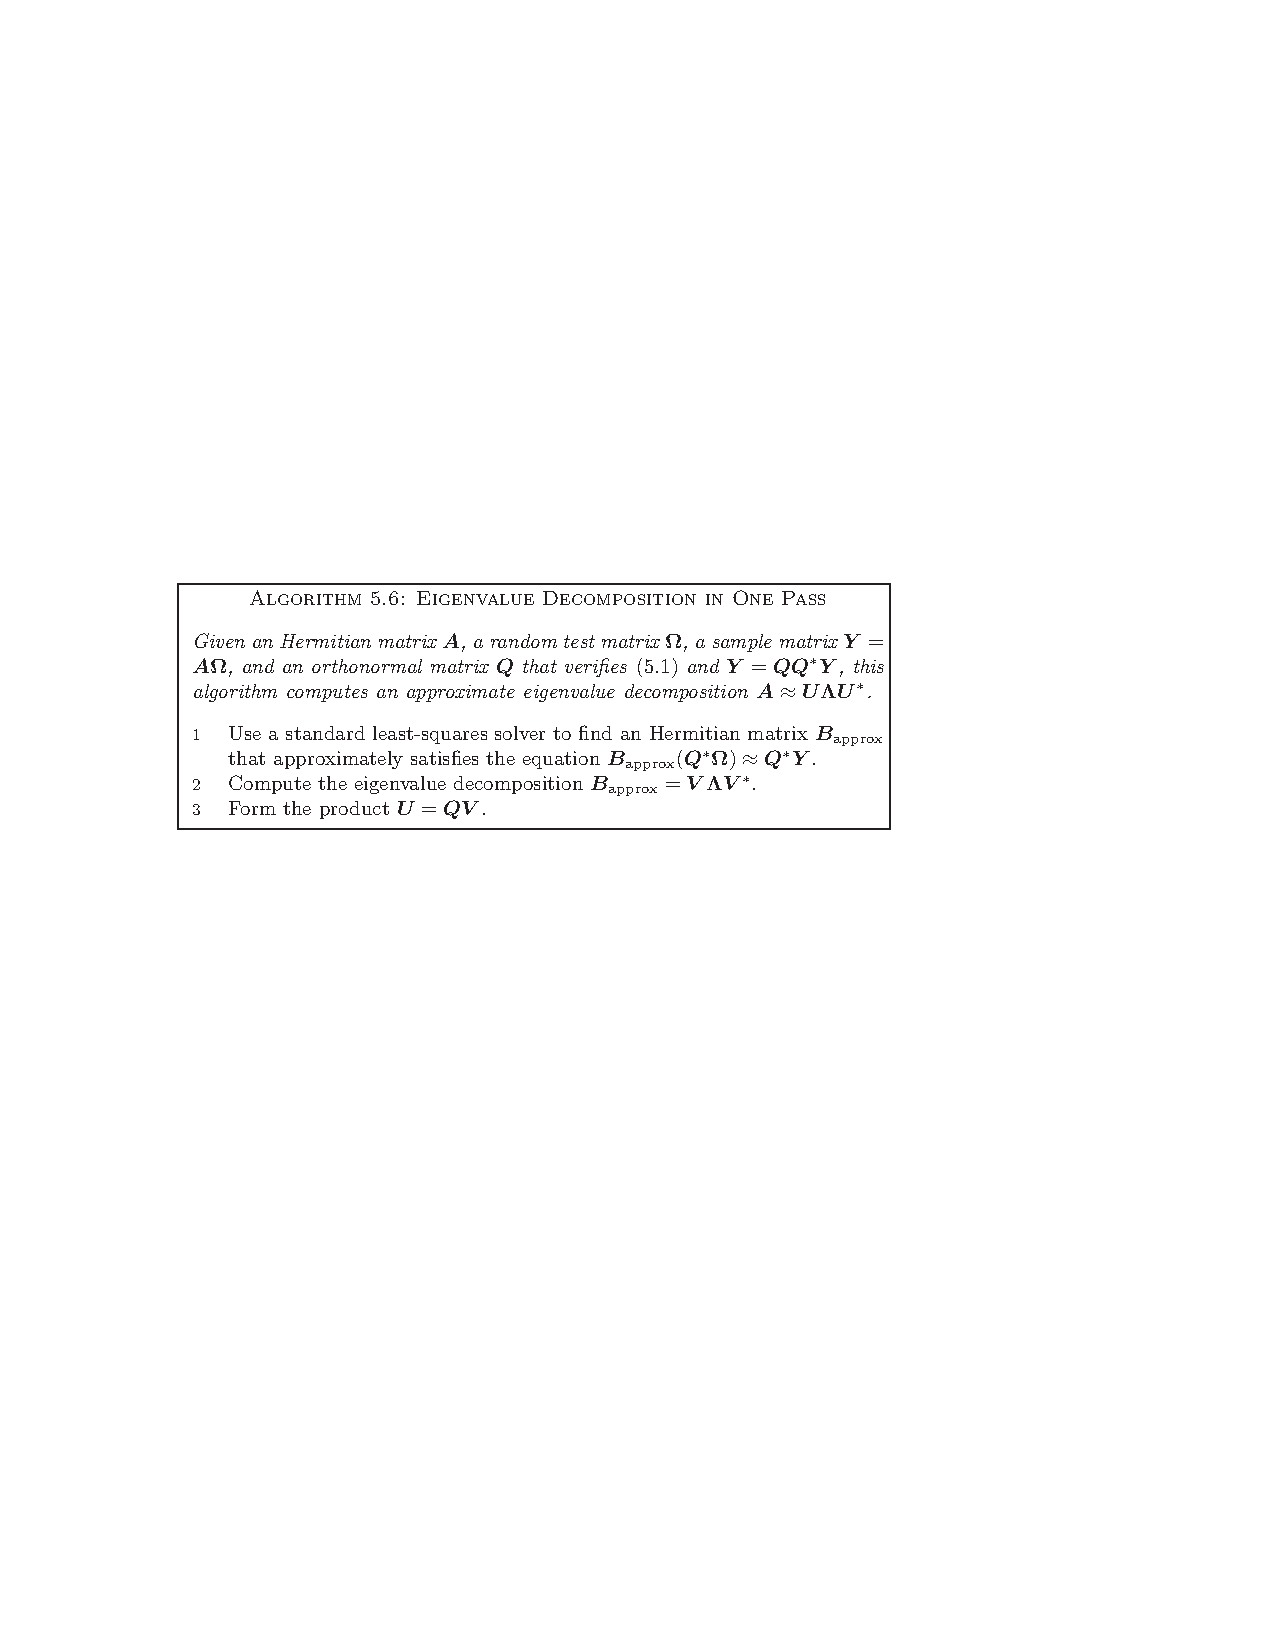
\includegraphics[height=5.5cm]{../graph/singlepass-eps-converted-to.pdf}
\end{center}

\section{Results and Discussion}

This section will compare the speed of running MATLAB's default eig function against the power iteration, rayleigh iteration, and single pass algorithms on various types of square matrices, ranging from $100 \times 100$ to $ 2000 \times 2000$, in increments of 100. Additionally, the ratio between the largest and second largest eigenvalues of the matrices are plotted to give an idea of the convergence of the power iteration based algorithms. The single pass algorithm samples all n rows of the matrix. In the following section, we will vary the amount of rows sampled in order to examine the tradeoff between accuracy and speed. 

The results of the inverse iteration algorithm were not included because it was outperformed by the rayleigh iteration algorithm. Moreover, in order for it to converge to the desired eigenvalue, the eigenvalue approximation must already be quite close to the correct answer.

\subsection{} \textbf{Random Normal Hermetian Matrix.}

\begin{center}
\epsfig{file=../graph/randn/"time elapsed alt".eps, height = 8cm}
\end{center}

The above graph shows the results of running the power iteration, rayleigh iteration, and single pass algorithm on normally distributed hermetian matrices. The default eigenvalue solver in matlab gave the fastest results, which was to be expected as the difference between the largest eigenvalue and second largest eigenvalue was very small. On the other hand, the power iteration, rayleigh iteration, and single pass algorithms were all very erratic. In the normally distributed case, with eigenvalues that are clustered closely together, the power iteration based algorithms are not a very good choice.

\begin{center}
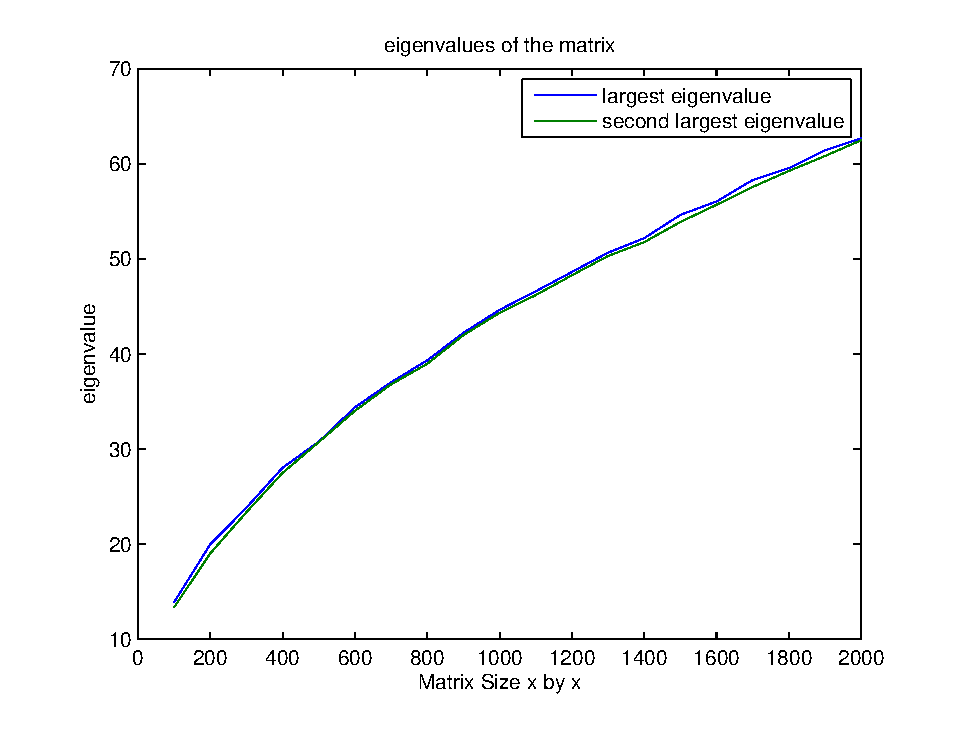
\epsfig{file=../graph/randn/eigenvalues.eps, height = 8cm}
\end{center}

As can be seen, the largest eigenvalue and second largest eigenvalue are very similar in size. This explains the slow convergence of the power iteration algorithm.

\subsection{} \textbf{Random Uniform Hermetian Matrix.}

\begin{center}
\epsfig{file=../graph/rand/"time elapsed alt".eps, height = 8cm}
\end{center}

The above graph shows the results of running the power iteration, rayleigh iteration, and single pass algorithm on uniformly distributed hermetian matrices. Unlike the normally distributed matrices, the dominant eigenvalue is much larger than the second largest eigenvalue. As a result, the power iteration algorithm converges much faster compared to the normal case. Similarly, Rayleigh iteration is comparable to the default eigenvalue solver. However, the single pass algorithm is still the slowest of the algorithms.

\begin{center}
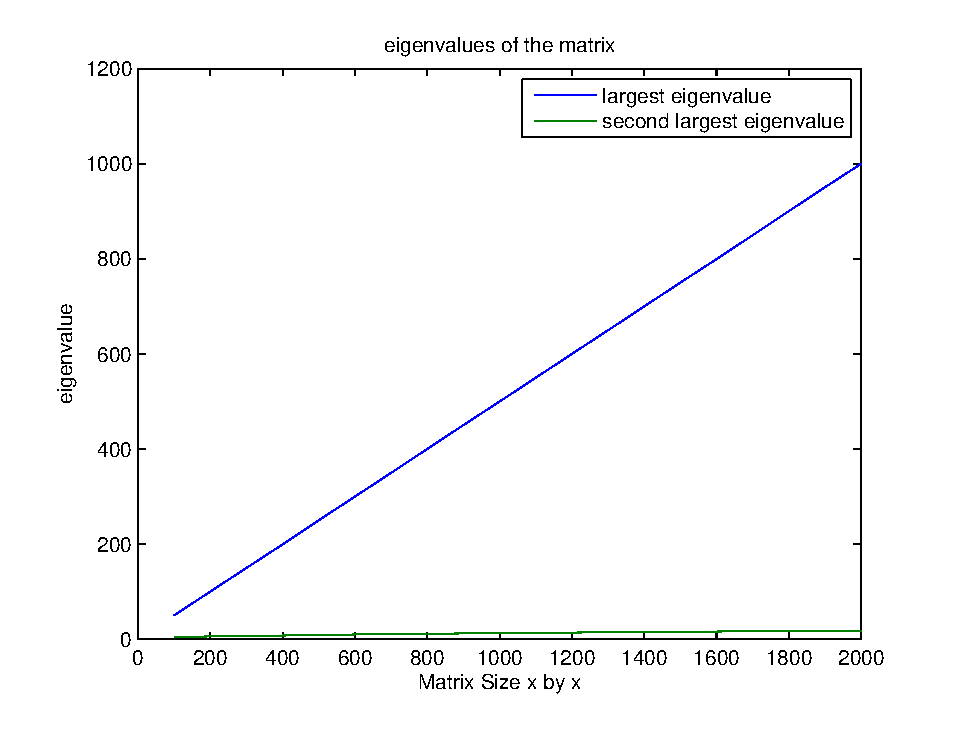
\epsfig{file=../graph/rand/eigenvalues.eps, height = 8cm}
\end{center}

As can be seen, the difference between the two eigenvalues are very large. As a result, the power iteration algorithm converges quickly.

\subsection{} \textbf{Sparse Hermetian Matrix.}

\begin{center}
\epsfig{file=../graph/hermetiansparse/"time elapsed alt".eps, height = 8cm}
\end{center}

The above graphs shows the results of running the power iteration, rayleigh iteration, and single pass algorithm on sparse hermetian matrices, with a $95\%$ chance of containing zero, and a $5\%$ chance of containing one. This type of matrix can be used to represent an undirected graph. If there is a one at index $(i,j)$, then there is a connection between the $ith$ and $jth$ position vertices of a graph. As can be seen, the results are very similar to the uniformly distributed case, with the exception that the rayleigh iteration method is slightly slower than in the uniform case.

\begin{center}
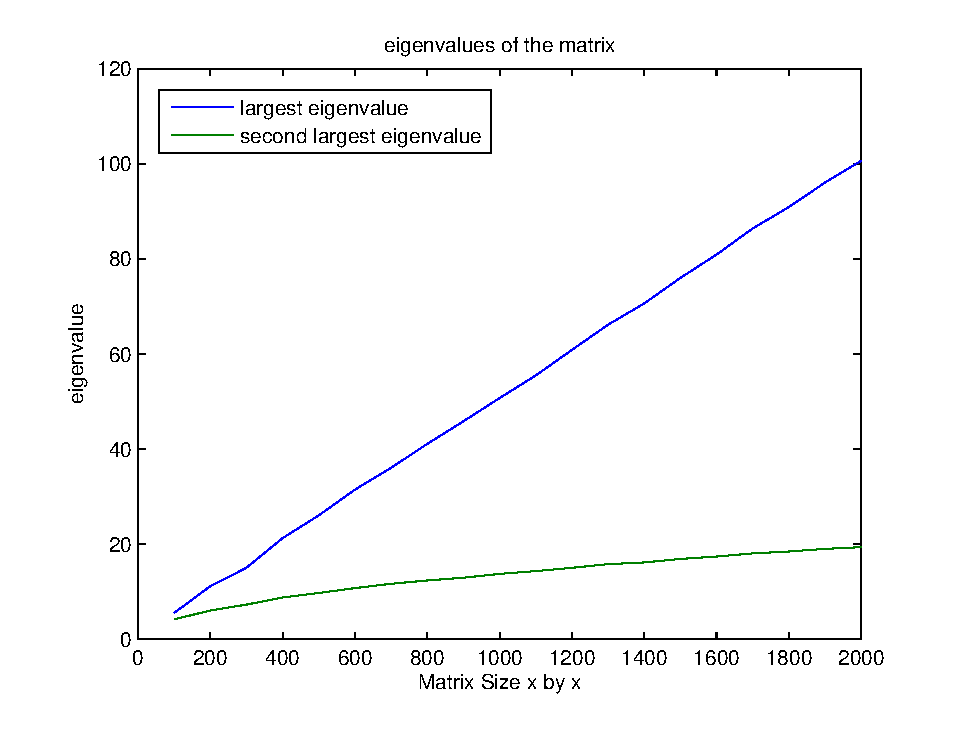
\epsfig{file=../graph/hermetiansparse/eigenvalues.eps, height = 8cm}
\end{center}

Again, there is a wide gap between the largest and second largest eigenvalues in the matrices.

\subsection{} \textbf{Sparse Non Hermetian Matrix.}

\begin{center}
\epsfig{file=../graph/nonhermetiansparse/"time elapsed alt".eps, height = 8cm}
\end{center}

The above shows the results of running the power iteration, inverse iteration, rayleigh iteration, and single pass algorithm on sparse matrices, with a $5\%$ chance of containing a one, and a $95\%$ chance of containing a zero. This type of matrix can be used to represent a directed graph, with a one representing a one-way connection between the $ith$ and $jth$ position vertices of a graph. The results are again similar to the uniform distribution, although the default MATLAB eig function is outperformed by both the rayleigh and single pass algorithms, as well as the power iteration algorithm.

\begin{center}
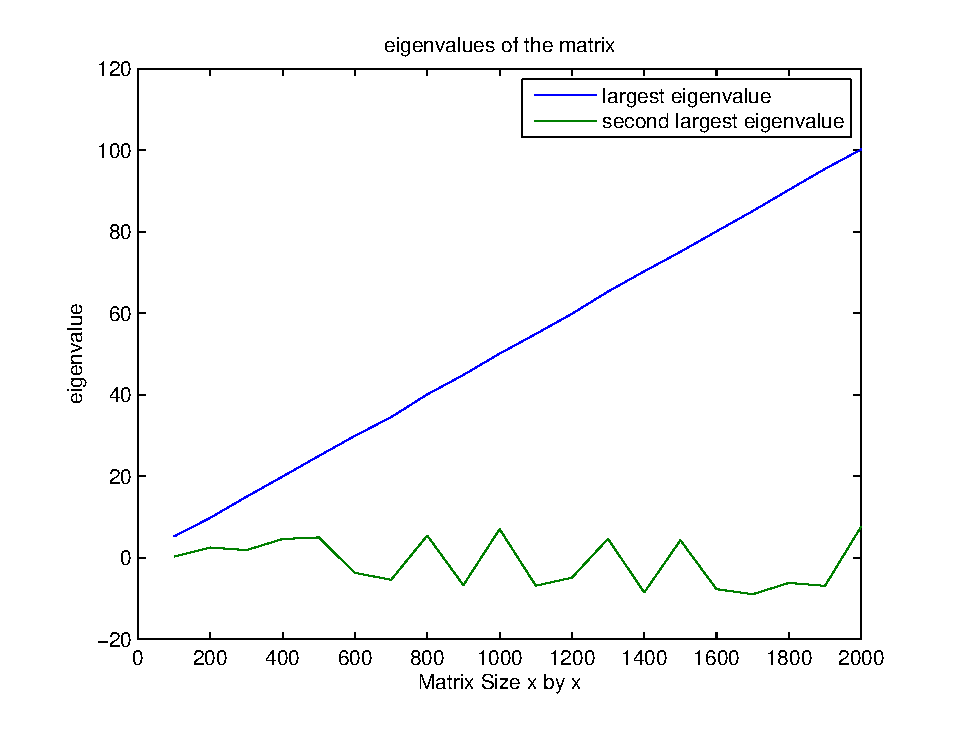
\epsfig{file=../graph/nonhermetiansparse/eigenvalues.eps, height = 8cm}
\end{center}

From these examples, we see that if there is a large gap between the largest eigenvalue, and the second largest eigenvalue in the matrix, the power iteration algorithm converges quite quickly, and is quite a bit faster than the default MATLAB eig function. However, if the ratio between the largest eigenvalue and the second largest eigenvalue is close to one, then the algorithm converges extremely slowly.

\section{Applications and Example}

%\subsection{}



\end{document}  